\documentclass[aspectratio=169]{beamer}
%% For 4:3 aspect ratio:
%% \documentclass{beamer}
\usepackage{../git-course}

\title[git-course]{An Introduction to \gh\ and \gs}
\author{Andrew Edwards}
\date{\today}

\begin{document}
%% Needed to remove 'Figure:' from figure captions:
\setbeamertemplate{caption}{\raggedright\insertcaption\par}

\frame[plain]{
\titlepage
}

\section{Introduction}

\frame{\frametitle{Basics}
  \bigskip
  June 2021 testing:
  ~\\
  I will go through the next slides up to slide 9, demonstrating the basic commands.\\
  ~\\
  Some are only needed once per repository to get set up.\\
  ~\\
  So first sit back and listen, then go back through the slides yourself following the
  instructions, to become familiar with the basic ideas.\\
  ~\\
  Then you can do the Exercise on page 10.
}

\section{Creating/Cloning}
\frame{\frametitle{Creating a new repository}
  \bi
    \item Sign into your \gh\ account, click on the
      \emph{Repositories} tab, and press the \emph{New} button.
    \item Give your repository a name. Let's call it \lst{test}.
    \item Check \emph{Initialize this repository with a README}.
    \item Leave \emph{`Add .gitignore`} and \emph{`Add a license`}
      set to \emph{None}.
    \item Click \emph{Create repository}.
  \ei
}

\frame{\frametitle{Cloning your new repository}
  \bi
    \item Now copy the full URL of your test repository.
    \item Open the \gs\ and run the following command to \emph{clone} your repository:
      \lst{git clone URL}\\
      where \lst{URL} is the url of your newly created repository. You
      can paste the \lst{URL} into the command line (on Windows) by
      pressing the right mouse button.
  \ei
  \bigskip
  You should now have a subdirectory called \lst{github/test} on your computer.\\

  In \gs, change
  to that directory:\\
  \lst{cd test}
  ~\\
  So `clone' is Git speak for copying something from GitHub onto your local
  computer.
  ~\\
  This example has just one file (the README). But the process is the same for a
  repository with multiple files and multiple directories (the structure is
  fully preserved).
}

\frame{\frametitle{Windows only: Storing your credentials [TODO: not sure about
    this nowadays]}
  When you are using the \gs\ for the \alert{very first time}, issue
  the following command:\\
  \bigskip
  \lst{git config --global credential.helper wincred}\\
  \bigskip
  This means that you don't have to repeatedly enter your \gh\ password.\\
  The command creates a credential file containing your account information:\\
  \lst[escapechar="\\"]{C:\\Users\\YOUR-COMPUTER-USER-NAME\\.git-credentials}\\
}

\section{Committing new files}
\begingroup
\small
\frame{\frametitle{Copy and commit \emph{.gitignore}}
  \bi
    \item Copy the \emph{.gitignore} file from the \lst{module-1-git/git-intro}
        directory that you should have already from the setup talk, and
      paste it into your new \lst{github/test} directory. (We are using
      \emph{.gitignore} as an example file here). TODO: simplify? ``Create new-file.txt''?
    \pause
    \item Check the status of your (\lst{test}) repository: \lst{git status}
    \pause
  \item It should say that you have an `Untracked file' called \emph{.gitignore}.
      You want to tell Git to start tracking it, by using the \lst{git add}
      command:\\
      \lst{git add .gitignore}
   \pause
 \item Type \lst{git status} again.
 \item You should see that the file is listed as a `new file` under `Changes to
   be committed`.
    \item Let's now `commit' it:\\
      \lst{git commit -a -m "Add .gitignore file."}\\
      The commit message should be a useful message saying what the commit
      encapsulates.\\
    \pause
    \item Push the commit to \gh: \lst{git push}
    \pause
    \item Check (refresh) the \gh\ webpage and see your commit and the uploaded file.
  \ei
}
\endgroup

\frame{\frametitle{What just happened?}
  We just used three of the main Git commands:
  \bi
  \item \lst{git add <filename>} -- tell Git to start keeping track of changes
    to this file. You only need to tell Git this once.
  \item \lst{git commit -a -m "Message."} -- committing your changes, which means tell Git
    you are happy with your edits and want to save them. % You are actually saving
    % a snapshot of your entire repository (all the folders and files in your repository).
  \item \lst{git push} -- this sends your commit to the GitHub website.
  \ei
  ~\\
 You always have your files stored \emph{locally} on your computer. When
    you push to GitHub they can then be easily fetched (retrieved) by whoever
    you are collaborating with.
}

\frame{\frametitle{Keyboard aliases (shortcuts)}
Now, \lst{git commit -a -m "Message."} is a bit much to type, so we have an
alias for it:

~\\

\lst{git com "Message."}

~\\

This is defined in the \emph{.gitconfig} file you installed in the `git-setup`
instructions.

~\\

The \lst{-a} means `commit all changes of files that Git is tracking`, and \lst{-m} is
to include a message. Since we usually want to do both of
these, \lst{git com "Message."} is a useful shortcut. But it is important to
realise it is an alias if searching online for help.

Similarly:

\lst{git s} -- for \lst{git status}

\lst{git p} -- for \lst{git push}

From now on we will use the aliases.

TODO: say how to simplify to \lst{g s} etc. W: from Chris.
}

\frame{\frametitle{Edit \emph{Readme.md}}
  Edit the \emph{Readme.md} file. Add some simple comments describing
  the project such as: ``A test repository for learning Git.''\\
  \bigskip
  \pause
  Look over the changes, commit them, and push them to your \gh\
  repository:\\
  \lst{git s}\\
  \lst{git diff} -- this shows the differences between the last committed
  version and your current version (of all files; only one in this case) \\
  \lst{git com "Initial edit of Readme.md"}\\
  \lst{git p}\\
  ~\\
  Refresh your \gh\ web page and you should see your text
  (the \emph{Readme.md} file is what is shown on the main page
  of your repo).
}

\frame{\frametitle{Exercise: copy, edit and commit \emph{simpleText.txt}}
  \bn
    \item Copy the text file \lst{module-1-git/exercise-files/simpleText.txt}
      into your local \lst{test} repository.
    \pause
    \item Predict what \lst{git s} will tell you, \emph{then} type it in the
      Git shell to check.\\
    \item Add the file to the repository using the git commands:\\
      \lst{git add simpleText.txt}\\
      \lst{git s} -- not necessary but useful to check you understand what is
      changing before you commit\\
      \lst{git com "Adding simpleText.txt"}\\
      \lst{git p}
    \pause
    \item Do some editing of simpleText.txt (see instructions at start of
      it), to get the hang of \lst{git com} and \lst{git p}.
    \pause
    \item \lst{git com "Message"} frequently and \lst{git p}
      occasionally, while intermittently doing \lst{git s} and
      \lst{git diff} to understand what's changing.
    \pause
    \item Keep an eye on your commits by refreshing the \gh\ page.
  \en
}

\frame{\frametitle{Adding multiple files at once -- slide 1}
  Often you add multiple files in a new directory. When you run \lst{git s}, you
  will see a large list of \emph{Untracked files}. They can be added at once by simply
  adding the whole directory.
  \bi
    \item Create a new directory to your \lst{test} repository, using your normal method. Call it \lst{new-stuff}.
    \item Add a few new test files to that directory called
      \lst{test1.txt}, \lst{test2.txt}, etc. Put some example text
      in one or more of them if you want.
    \item On the command line, check the status:\\
      \lst{git s}
    \item You will see a listing showing the \emph{new-stuff} directory in
      \emph{Untracked files}.
%    \item To see the actual files to be committed instead of just the
%      directory:\\
%      \lst{git s -u}
    \item To add all the new files in preparation for a commit,
      issue the command:\\
      \lst{git add new-stuff/}
  \ei
  \bigskip
  Continued...
}

\frame{\frametitle{Adding multiple files at once -- slide 2}
  \bi
    \item Check the status of the repository again:
      \lst{git s}
    \item It will now show all files in \emph{Changes to be committed}
    \item Commit the changes:\\
      \lst{git com "Added new-stuff directory."}
    \item Push the changes to \gh:\\
      \lst{git p}
    \item Check your \gh\ webpage and see your commit and that the files
      have been uploaded.
    \item That works no matter how many files are in your \lst{new-stuff}
      directory.
  \ei
}

\frame{\frametitle{Adding multiple files at once -- slide 3}
  \bi
    \item To add multiple files with similar names you can use the wildcard
      \lst{*} symbol.
    \item You just added (told Git to keep track of) the new files in your
      \lst{new-stuff/} directory.
    \item If you add more new files to that directory, you will
      have to tell Git to track those also (since they are new -- you haven't
      told Git about them yet).
    \item Say you have 10 new files called \lst{idea1.txt}, \lst{idea2.txt}, ..., \lst{idea10.txt}.
    \item Instead of typing\\
      \lst{git add idea1.txt}\\
      \lst{git add idea2.txt}\\
      etc.
      you can just use the wildcard \lst{*}:\\
      \lst{git add idea*.txt}\\
      (or even just \lst{git add *.txt}, or \lst{git add *.*}).
  \ei
}


\frame{\frametitle{The \emph{.gitignore} file}
  But what if you don't want to add all the files that you create?

  Each repository can have a \emph{.gitignore} file, in the root directory
  of the repository. This file has names of files or wildcard names such as
  \lst{*.pdf} or \lst{*.doc} or \lst{my-secret-notes.txt} that will be completely ignored by \gs.

  Some programs you run may make temporary files that don't need to be tracked
  by Git, the names of which should also be added to \emph{.gitignore}
  adding these files when adding whole directories
  using commands such as \lst{git add new-stuff/}.\\
  \bigskip
  This is important as you will clutter up your repository and have to spend
  time cleaning it all up.\\
  \bigskip
  When you run \lst{git s} you may see untracked files that you don't want to be tracked
  (they are fine on your computer but Git won't keep track of them or push them
  to \gh). You should add them or a wildcard template encapsulating them to the
  \emph{.gitignore} file so that they are not added inadvertently.
}

\frame{\frametitle{Renaming files}
  \bi
    \item You can rename any files the way you usually would (e.g. in File Explorer).
    \item Once you've renamed your files, check the repository status:\\
      \lst{git s}\\
    \item You will see that the files you renamed have been automatically
      deleted from the repository and need to be added again. Do this the
      same way you add new files (\lst{git add filename}). You can also
      add a whole directory again and \gs\ is smart enough to only add the
      renamed files.
    \item Check the status again:\\
      \lst{git s}\\
      It will show that the file(s) were renamed.
    \item Make a commit:\\
      \lst{git com "Renamed files x, y, and z"}\\
    \item Push the commit:\\
      \lst{git p}
  \ei
}

\frame{\frametitle{The power to go back}
  With Git you can revert back to any previous state of your repository.\\
  This is {\red very powerful}, though slightly {\red scary} at first.
  \bn
    \item \lst{git s} to make sure you are all up-to-date
      (\lst{commit} and/or \lst{push} if necessary).
    \item In File Explorer (or whatever) look at your repository.
    \item Look at the commit tab on \gh\ for your \lst{test} repo and copy
      the first five digits of the \lst{HASH} to the clipboard.
    \item In \gs, do\\
      \lst{git checkout HASH}
    \item Look at File Explorer again -- your \lst{new-stuff} directory should
      have ... disappeared!!\\
      (If it hasn't then open it -- the test files, i.e. \lst{test1.r}
      , \lst{test2.r}, etc. should be gone, but your text editor may
      have saved backup versions; manually delete them plus the
      \lst{new-stuff} directory)
    \item You are now back to the very first version of your repo.
  \en
}
\frame{\frametitle{Back to the latest version}
  Now, to get your files back to the most recent version you had committed:
  \bi
    \item \lst{git checkout master}
  \ei
  \bigskip
  That's it. So you can {\red revert to any previous commit in your
    repository}.\\
  \bigskip
  Very reassuring, especially for complex code that you may mess up and just
  want to go back to yesterday's version.\\
  \bigskip
  We will take a closer look at this in the advanced section, as there
  are several things you can do once you go back to a previous commit.\\
  \bigskip
  In practice you rarely actually revert back, but it's comforting to know
  that you can.
}

\frame{\frametitle{Versions}
  Transiting the commit history is less cluttered and more tractable than:
  \centering
  \begin{figure}
    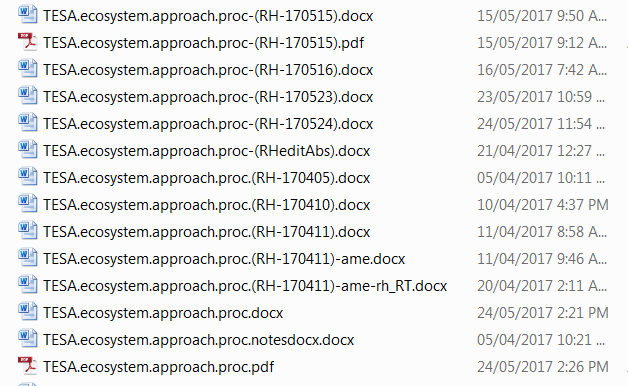
\includegraphics[
        width=\textwidth,
        height=0.8\textheight,
        keepaspectratio]
        {../git-motivation/figures/EAversions.png}
      \end{figure}

TODO Somewhere: Note that you still edit and save your files in the usual way. If you don't commit you will still have the latest versions of your files on your computer
  (as you would if you weren't using Git).

}

\frame{\frametitle{So how does Git do all that?}
  \bi
    \item By now you're probably wondering how Git keeps track of everything.
    \item There is a hidden \lst{.git} directory in each repository.
    \item Look at the \lst{objects} subdirectory. Each subdirectory name is the
      first two digits of a hash. The rest of the hash are the names in the
      directory. The hashes represent \textbf{file contents (blobs)},
      \textbf{commits},
      and \textbf{directory structures (trees)}.
    \item Because of these structures, you can go back and {\red rebuild} any
      or all files at any \lst{commit}, and even have different directory
      structures at each commit.
    \item Works best for ASCii (text) files, such as \lst{.R}, \lst{.txt},
      \lst{.Rmd}, \lst{.Rnw}, etc.
    \item Works for binary files, e.g. \lst{.RData} and \lst{.xls} files but
      you will not be able to do any useful merging with those files. You will
      lose the power that git provides.
    \item Exceptions: Image files that aren't likely to change. There are some
      in the \lst{git-course} repository.
  \ei
}

\frame{\frametitle{Commits and history}
  Git does not keep versions of code, it keeps \emph{commits}. The commits
  are kept track of using a hash code, using \emph{Secure Hash Algorithm 1}
  (SHA-1) which generates a hash key 40 digits long in hexadecimal. These are
  what you see on \gh\ and in various places when you use \gs.\\
  \bigskip
  Several of these commits have pointers to them which have special names:
  \bi
    \item The \textbf{HEAD} which points to the commit you are currently on
      in the \gs.
    \item The \textbf{master} which is just the default branch when you set
      up a repository on \gh.
    \item The branch names that you have in your repository.
  \ei
  Once you've cloned a \gh\ repository, the \textbf{master} points to the initial
  commit, and the \textbf{HEAD} points to the master.\\
}

\frame{\frametitle{Thoughts/hints regarding commit messages}
  What to write in \lst{git com "Message"}?\\
  Ideally:
  \bi
    \item Want to describe \emph{what} and (sometimes \emph{why}) you did
       something.
    \item The \emph{how} is not needed since that will be explained by the
       actual changes in the code.
    \item Message should be informative for collaborators (including your future self).
  \ei
  {\red Bad}:\\
  ~~\lst{git com "Tweaked function."}\\
  {\blue Good}:\\
  ~~\lst{git com "Allow plot.biomass() to use extra colours."}\\
}

\frame{\frametitle{Why you should not commit binary files}
  An example:
  \bi
  \item A collaborator had added \lst{.pdf}, \lst{.RData} and \lst{.docx} files
     (plus \lst{.R} etc.), but these got updated when the code was run.
  \item Git has to save every version of each of these binary files even if just
    one word has been changed.
  \item I ended up with \lst{.git/objects/pack} being 2.8Gb.
  \item I needed space quickly so just deleted four files in
     \lst{.git/objects/pack}, which freed up 1.6Gb.
  \item Note that I still have the actual final versions of files (as you would
     if not using Git), but just not the full repository history.
  \item However, when I tried to later do some work and then \lst{commit} I got ...
  \ei
}

\frame{\frametitle{Why you should not commit binary files}
  \centering
  \begin{figure}
    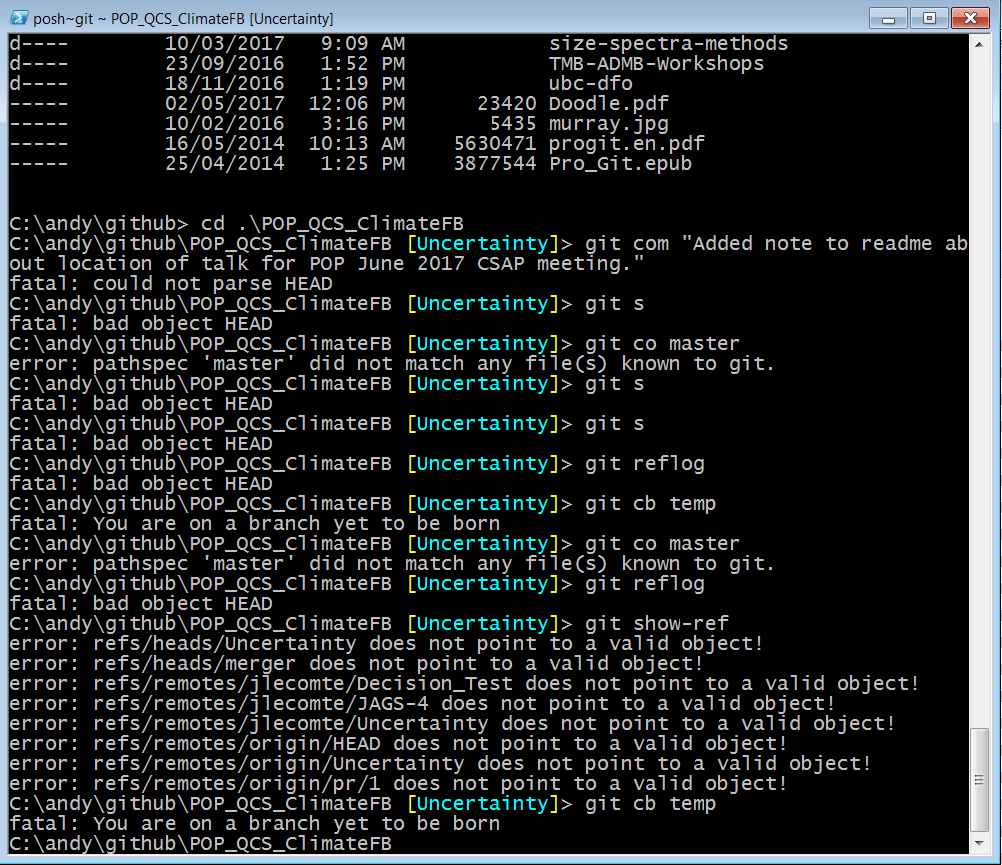
\includegraphics[
        width=\textwidth,
        height=0.8\textheight,
        keepaspectratio]
        {../git-motivation/figures/notGood.png}
  \end{figure}

  \textbf{\large Don't mess with the .git directory!!}
}

\section{Branches}
\frame{\frametitle{Branching overview}
  When you want to add some new code to your project, but don't want to break
  what is already there, you create a new branch. When creating a new branch,
  your starting point is identical to the branch you were in when you created
  the new one.\\
  \bigskip
  Once you have completed your work in the new branch and are satisfied that
  everything is working correctly, you merge the changes into your master
  branch (or any other branch you wish).\\
  \bigskip
  You can also push branches to \gh\ if you feel the branch is going to be a
  longer term project and/or if there are going to be multiple collaborators
  on that new branch.\\
  \bigskip
  It is a good idea to commit all changes before creating a new branch, as
  local changes which haven't been committed will appear in the new branch
  as well.
}

\frame{\frametitle{Creating a new branch}
  \bi
    \item In the \gs, enter your test repository:\\
      \lst{cd test}\\
      and see that you are in the \emph{master} branch by looking at the
      prompt.
    \item Create a new branch based off the branch you are currently on:\\
      \lst{git checkout -b temp}\\
      You will be automatically placed in the new branch called
      \emph{temp}, and commits you make will now occur in that
      branch only.
    \item To view all local branches:\\
      \lst{git branch}\\
      There is an asterisk next to the branch you are currently in.
    \item To switch to another branch, let's say back to \emph{master}:\\
      \lst{git checkout master}\\
  \ei
}

\frame{\frametitle{Make a commit in the new branch}
  \bi
    \item Make sure you are in the new branch:\\
      \lst{git checkout temp}
    \item Create a new file called \lst{tester.txt}
    \item \lst{git add tester.txt}
    \item \lst{git com "Added tester.txt"}
    \item Switch back to \emph{master}:\\
      \lst{git checkout master}
    \item Notice that the file you just added is gone. It only exists in
      the \emph{temp} branch at this point. You will need to merge that
      branch back in to the \emph{master} branch if you want to keep the
      work you did in the other branch.
  \ei
}

\frame{\frametitle{Merging branches}
  \bi
    \item To merge the changes from a branch into another branch:
      \bn
        \item Change to the branch you want to merge into, typically
          \emph{master}:\\
          \lst{git checkout master}
        \item Merge the branch into \emph{master}:\\
          \lst{git rebase temp}\\
          OR\\
          \lst{git merge temp}
      \en
    \item Notice that the file you created in the \emph{temp} branch
      now appears in the \emph{master} branch. All commits done in a branch
      which is merged in will be included in the merge step.
    \item If there was a merge conflict, you must fix it at this point. This
      will be covered later in the section about merging remotes, which
      follows the exact same method.
    \item Since we are done with that branch for good, we will delete it so
      we don't have unused branches hanging around (next slide).
  \ei
}

\frame{\frametitle{Deleting branches}
  \bi
    \item To delete a branch that you are not currently in, in this case
      the \emph{temp} branch:\\
      \lst{git branch -d temp}\\
    \item To delete the branch you are currently in, switch to another branch
      first, (e.g. \emph{master}) and then delete the branch:\\
      \lst{git checkout master}\\
      \lst{git branch -d temp}\\
    \item If you have unmerged changes in the branch, you will not be allowed
      to delete it. If you want to forcibly delete it, discarding your changes,
      use:\\
      \lst{git branch -D temp}\\
      \textbf{Warning -- you won't be able to get any of those changes back
        once you do this.}
  \ei
}

\frame{\frametitle{Pushing branches to \gh}
  If you want to push the branch up to \gh, i.e. so others can fetch it and
  edit it, you need to be in the branch locally and:\\

  \lst{git --set-upstream origin BRANCH-NAME}\\

  \gs\ is smart, so if you forget this command and instead type:\\

  \lst{git p}\\

  while in the new branch, \gs\ will tell you the command you need.\\
  \bigskip
  Once you've done this for a branch, all you have to do to push future
  commits in this branch is:\\
  \lst{git p}\\
  \bigskip
  Check the \gh\ webpage to see that your branch was pushed.
}

\frame{\frametitle{Deleting branches from \gh}
  To remove a branch entirely from \gh:\\
  \lst{git p origin --delete BRANCH-NAME}\\
  \bigskip
  The local branch will still exist, so if you want to delete that as well:\\
  \lst{git checkout master}\\
  \lst{git branch -d BRANCH-NAME}
}

\section{Git Workflow}
\frame{\frametitle{Git Workflow}
  There are two ways to work using Git and \gh:

  \bn
    \item A project where people contribute to a main repository that is
      considered the 'master copy'.
      \bi
        \item Don't fork, instead clone directly from the creator's repository.
        \item All collaborators require push access to the main repository
      \ei
    \bigskip
    \item A project where collaborators fork from an initial repository so that
      each have a copy of the repository, none of which are the `master copy'.
      \bi
        \item Fork a copy from the initial creator's repository.
        \item Merge other people's remote repositories into yours using \gs.
        \item Each collaborator can send a \emph{Pull request} to the creator on the
          \gh\ site. They accept your pull request and your code is merged into
          the `master copy'.
        \item This stops other people messing up your `master copy'.
      \ei
  \en
}


\frame{\frametitle{Demonstration of collaborating}
  \bi
    \item Andy to clone Chris's \lst{test} repo.
    \item Chris gives Andy `push access' to his \lst{test} repo.
    % \item Both add each other as remotes.
    \item Both do some edits (Andy create new files, Chris edit existing ones).
    %  keeping an eye on the evolving Network Graphs.
    \item (This might not be 100\% right -- we'll update in the workshop):
      For Andy to get Chris's updates (and vice versa), it will just be:
    \bi
      \item \lst{git fetch}
      \item \lst{git rebase} OR \lst{git merge}
      \item \lst{git p}
    \ei
  \ei
  %\bigskip
  %It's actually even easier because \lst{git} will autocomplete, so
  %  Andy can just do \lst{git fetch c<TAB>} etc.
}

\frame{\frametitle{Exercise on collaborating on a single repository}
  \bn
\item Each group of four sitting together will collaborate. Each group
  will choose one person to create the repository.
    \item The chosen person will set up a new repository on \gh\ called
      \lst{help-friends}
    \item The chosen person copies \lst{git-course/exercise-files/helpFriends.txt}
      into their new repository (on their computer).
    \item \lst{add}, \lst{commit}, \lst{push}.
      Check Network Graph.
    \item The chosen person gives permission to the others to collaborate for their
      repository on \gh.
    \item The other three people then clone the repository using Person 1's URL.
    \item Everyone does a few edits on their paragraph number only.
      (see \lst{helpFriends.txt}).
    \item \lst{commit} a few times, \lst{push}.
    \item If server does not allow you to push: \lst{git fetch}, \lst{git rebase}, \lst{git p}
  \en
}


\section{Network Graph}
\frame{\frametitle{Network Graph}
  \bi
     \item The Network Graph is a useful visualization tool to keep
       track of your commits.
     \item Each \lst{commit} is shown as a point on the graph.
     \item Hover the mouse over a commit to see:
     \bi
       \item who committed
       \item the commit \lst{HASH} -- a 20-byte hexadecimal string that
         identifies that commit;\\
         e.g.: \lst{1ef1da5659a4b147562b155ffb6289811adab36b}
       \item the commit message (so provide meaningful messages!).
     \ei


     \item Click on a commit to see the actual changes made for that commit
        (therefore commit frequently so each commit only has a few changes).
     \item See that you (or a collaborator) can add comments for each commit.
     \item In the comments (or when you do \lst{git commmit -a -m "..."}) you can include
        a \lst{HASH} from any other commit. You only really need the first five
        digits to ensure uniqueness ($16^5 = 1,048,576$ possible combinations),
        but if you use seven then \gh\ will create a link to that commit
        (see June 13th commits).
  \ei
}

\frame{\frametitle{Understanding the Network Graph}
  The Network Graph is useful when working alone, but especially so when
  collaborating using forking (which we haven't really shown, so we'll
  only talk about some of these slides).\\
  \bigskip
  Find it for any repo under \lst{Insights-Graphs-Network}.\\
  \bigskip
  Look at \url{https://github.com/cgrandin/git-course/network}\\
  \bigskip
  Hover over commits to see commit details.\\
  \bigskip
  Hints for \gh:
  \bi
    \item \gh\ has keyboard shortcuts. Type \textbf{?} while on the site
      to get a list of them.
    \item Use left and right arrows to navigate the network graph.
    \item Use shift-left arrow or shift-right arrow to go to the beginning
      or end of the network graph.
  \ei
}

\frame{\frametitle{Understanding the Network Graph}
  Screenshot from 30th May shows (and next page):
  ~\\
  ~\\
  \includegraphics[
     width=\textwidth,
     height=0.6\textheight,
     keepaspectratio]
     {../git-motivation/figures/netWorkGraph1}
}

\frame{\frametitle{Understanding the Network Graph}
  \includegraphics[
     width=\textwidth,
     height=0.6\textheight,
     keepaspectratio]
     {../git-motivation/figures/netWorkGraph2}

  Andy had done nothing for a while.

  [This is a slightly different way of collaborating to what we are now teaching].
}

\frame{\frametitle{Understanding the Network Graph}
  \includegraphics[
     width=\textwidth,
     height=0.6\textheight,
     keepaspectratio]
     {../git-motivation/figures/netWorkGraph1}\\
     The graph was for {\red Andy's repo}, so Andy is at the top.
     \\
  Chris's name shows up because he had pushed commits that Andy did not
    yet have.\\
  So the graph shows that Andy should get caught up before continuing on
    this project.\\
  This took three commands, resulting in:
  \includegraphics[
     width=\textwidth,
     height=0.6\textheight,
     keepaspectratio]
     {../git-motivation/figures/netWorkGraph3}
}



\frame{\frametitle{Understanding the Network Graph}
  \includegraphics[
     width=\textwidth,
     height=0.6\textheight,
     keepaspectratio]
     {../git-motivation/figures/netWorkGraph3}
  ~\\
  All files that Chris edited got updated, plus Andy then had any new files
    that Chris created, and our folder structures are identical.\\
  ~\\
  Chris's name doesn't show up, even though he did a lot of the work.\\
  ~\\
  It is ``{\red about code not ego}''.
  ~\\
}


\frame{\frametitle{Exercise regarding this git-course repo}
  \bn
    \item Look at {\red your} Network Graph for this \lst{git-course} repo.
    \item We'll look at some other people's.
    \item Why are they different?
    \item What to do?
  \en
}

\frame{\frametitle{Deleting or renaming remotes (may occasionally need)}
  \bi
    \item To delete someone as a remote:\\
      \lst{git remote rm REMOTE-NAME}\\
    \item To rename a remote:\\
      \lst{git remote rename OLD-NAME NEW-NAME}\\
    \item To see your changes, use:\\
      \lst{git remote -v}
  \ei
}

\begingroup
\small
\frame{\frametitle{Conflicts -- what if two people have edited the same lines?}
  The merge message will tell you which files are conflicting. Open those
  files one by one, and you will see the conflicted section bracketed like the
  following:\\
  \bigskip
  \lst{<<<<<<< HEAD}\\
  Line(s) of text/code which are currently in your file.\\
  \lst{=======}\\
  Line(s) of text/code which are trying to merge in, but conflict.\\
  \lst{>>>>>>> BRANCH-NAME}\\
  \bigskip
  where \lst{BRANCH-NAME} is the name of the branch you are trying to
  merge in from the previously-issued command:\\
  \lst{git merge BRANCH-NAME} ~~~e.g.~\lst{git merge cgrandin/master}\\
  All you do is remove the bracketing lines (\lst{<<<...} and \lst{>>>...}),
  the \lst{=======} line,
  and choose one of the line(s) of text/code to keep, or edit the line(s)
  to be something else entirely. Once you are done fixing each conflicted file,
  you need to \lst{add}, \lst{commit} and \lst{push}, e.g.:\\
  \lst{git add FILENAME}~~~(not quite sure why necessary, but \lst{git s}
    will remind you)\\
  \lst{git com "Kept Dave's edits as more consistent with
  remaining text."}\\
  \lst{git p}
}
\endgroup

\frame{\frametitle{Demonstration of conflicts}
  \bi
    \item Chris and Andy to carry on with existing repo
    \item Both modify {\red same lines of same file}
    \item Demonstrate how to rectify
    \pause
    \item {\bf Exercise:} Participants to create a conflict and fix
  \ei
}

\frame{\frametitle{\gh\ -- Add collaborators}
  If your \gh\ repository is public, anyone can post an \emph{Issue} (explained
    next). If you want someone to be able to:
  \bi
    \item set assignees to \emph{Issues}
    \item receive notifications when you reply to their \emph{Issue}
  \ei
  you need to add them as a collaborator. Select the \emph{Settings} tab and
    then the \emph{Collaborators} button. Type their \gh\ username in and send
    them an invitation to collaborate.
}

\frame{\frametitle{\gh\ -- Issues}
  \emph{Issues} are very useful for discussing issues with your repo.
  For this course we used them a lot:\\
  ~~\url{https://github.com/cgrandin/git-course}\\
  then click \emph{Issues}.\\
  ~\\
  Can see that we have some (maybe none?) `Open' -- still have not closed them.\\
  We have some `Closed' ones -- we have resolved the issue, maybe after a
    discussion.\\
  ~\\
  This is very useful and avoids having to clutter up code and write-ups with
    comments or endless emails that get overlooked.\\
  If an \emph{Issue} remains open you know that it hasn't been done.\\
  ~\\
  % Note that because Andy forked from Chris's repo, there is no \emph{Issues}
  %  page under\\
  % ~~\url{https://github.com/andrew-edwards/git-course}\\
}

\frame{\frametitle{\gh\ -- Issues}
  For hake we have over 430 closed \emph{Issues}:\\
  ~~\url{https://github.com/cgrandin/hake-assessment}\\
  ~\\
  Many of the unresolved ones are all tagged (using \emph{Milestones}) with
    `2019 assessment' -- not essential for finishing the 2018 assesssment but
    we didn't want to forget about them.\\
  ~\\
  You can assign collaborators to deal with an \emph{Issue}, and add comments.\\
  ~\\
  You automatically get emails when \emph{Issues} are created, commented on,
    etc.\\
  Equivalently, a blue notification circle appears on the bell at the top right
    (though I think it disappears when you read the email).\\
  ~\\
  Emails are useful, but if you're actively using your \gh\ page you can just
   turn them off (someone will know how ...).\\
  If you include the first seven digits of a commit \lst{HASH} it will become a
   clickable link.
}

\frame{\frametitle{\gh\ -- Issues}
  In your commit message you can refer to, say, Issue 41, using \#41.\\
  ~\\
  The commit then gets mentioned on the Issue page.
  ~\\
  Can even say something like\\
  ~~\lst{git com "Update catch figure, closes \#41."}\\
  ~\\
  This automatically closes the issue on \gh\, e.g.:\\
  ~~\url{https://github.com/cgrandin/hake-assessment/commit/0e88ff58}
    % bd6297cbdd6645a14219cf3d02edbae2}
}

\section{Undoing things}
\frame{\frametitle{Changing the commit message in the last commit}
  If you make a commit, then realize that your message had a spelling error,
  or needed more information in it, you can change the commit message:\\
  \bigskip
  \lst{git commit --amend -m "Correct message."}\\
  \bigskip
  This only works on the last commit. You can't change any other commit message
  using \emph{amend}.\\
  If you already pushed the commit before realizing that the message needs
  modification, do this:\\
  \bigskip
  \lst{git p --force}\\
  \bigskip
  after making the amendment to the commit message. You can also add more files
  before issuing the amendment commit and those files will be added to the commit
  you are amending. You can't add changes to file content this way though, you'll
  need to do another commit for that.
}

\frame{\frametitle{Undoing a commit}
  If you make a commit followed by other commits, then realize you want to undo
  the earlier commit, you use \emph{revert}:\\
  \bigskip
  \lst{git revert HASH}\\
  \bigskip
  where \lst{HASH} is the hash for the commit you want to undo (20-byte string)
  Remember that \gs\ is smart enough that you only need the first five digits:\\
  \bigskip
  \lst{git revert 1ef1d}\\
  \bigskip
  This actually creates a new commit with the automatic message\\
  ~~\lst{Revert "<previous commit message>"}.\\
  For example commit \lst{1fe84d4} in \lst{git-course}.\\
  \bigskip
  It is important to make a lot of commits, each with only small changes.
  You can only revert the whole commit, not parts.
}

\frame{\frametitle{Undoing changes not yet committed}
  If you've made a mess in your working directory and you want to change
  everything back to the way it was on the last commit:\\
  \bigskip
  \lst{git reset --hard HEAD}\\
  \bigskip
  If you've messed up a single file and just want that one file to go back
  to the way it was on the last commit:\\
  \bigskip
  \lst{git checkout HEAD file/to/restore.r}\\
  \bigskip
  Warning -- running these commands will delete the changes you have made.
  Since you have not committed any changes, they will be lost. Make sure
  you are certain you don't need the changes before running these commands.
  If you aren't sure if you need the changes again in the future, use
  \lst{git stash} instead.
}

\section{Stashing}
\frame{\frametitle{Stashing overview}
  If you are in the middle of working on something, but you need to change
  branches for some reason, you can \emph{stash} your changes and apply
  them back later. Let's say you are working in the master branch. To
  stash all changes in master:\\
  \lst{git stash}\\
  then change branches, and do whatever you like. To get those changes back,
  switch back to master:\\
  \lst{git checkout master}\\
  and apply the stashed changes:\\
  \lst{git stash pop}\\
  Note that nothing is committed, this just lets you put on hold your work
  in progress and come back to where you left off.\\
  \bigskip
  To make sure new files are included in the stash, you must have added them
  using \lst{git add filename} before using the \lst{git stash} command.
}

\frame{\frametitle{Stashing -- make it into a branch}
  If you leave a stash for awhile and have made commits since the stash,
  then try to reapply it, you may get conflicts. The best way to apply a stash
  if you have modified things since you stashed is to let git create a branch
  for the stash, which you can then look at and edit if you wish before merging
  back into your master or other working branch:\\
  \bigskip
  \lst{git stash branch BRANCH-NAME}\\
  \bigskip
  where \lst{BRANCH-NAME} is the name you want to call the new branch.
  You can then merge this branch in as outlined in the merging slides and
  resolve conflicts in the same way as with remotes or other local branches.
}

\section{Aliases}
\frame{\frametitle{Aliases}
  Are you getting tired of typing:\\
  \lst{git com "Message"} ?\\

  You can make your own shorter commands in git using Aliases. These are defined in:\\
  \bigskip
  \lst[escapechar="\\"]{C:\\Users\\YOUR-USER-NAME\\.gitconfig}\\
  \bigskip

  If you set up Git from scratch using our instructions you will already have
  that file that includes some of Chris's aliases. These include:

  \begin{table}
    \begin{tabular}{ll}
  \lst{git s}               & \lst{git status}\\
  \lst{git com "MESSAGE"}   & \lst{git com -a -m "MESSAGE"}\\
  \lst{git r}               & \lst{git remote -v}\\
  \lst{git cb BRANCH-NAME}  & \lst{git checkout -b BRANCH-NAME}\\
  \lst{git co BRANCH-NAME}  &  \lst{git checkout BRANCH-NAME}
    \end{tabular}
  \end{table}
These are on the readme file of this repo. Just remember (when Googling
problems) that these are aliases.
}

\section{Summary}
\frame{\frametitle{Summary}
  95\% of the time, this is all you are doing:\\
  \bigskip
  Change some source code\\
  \lst{git com "My commit message"}\\
  \lst{git p}\\
  If server does not allow you to push:\\
  \lst{git fetch}\\
  \lst{git rebase}\\
  If conflicts, fix them and:\\
  \lst{git add CONFLICTED_FILE}\\
  \lst{git rebase --resume}\\
  \lst{git p}\\
  \bigskip
  Change some source code...\\
  repeat... \\
}

\frame{\frametitle{Visualization website}
  Git Visualization website:
  \url{http://onlywei.github.io/explain-git-with-d3}
}

\frame{\frametitle{For tomorrow}
  You will need the TTT repo on your computer (it has some example code,
  plus then you'll also have the readme on your computer).\\
  \bi
  \item  In your git shell, make sure you are in your folder:\\
    ~~\lst{github/}
  \item Since you don't (all$^*$) have push access to \lst{pbs-assess/TTTworkshop}
    you need to:
  \item Fork it (on the \gh\ site)
  \item \lst{git clone http://github.com/YOUR-GITHUB-NAME/TTTworkshop}
    \ei
  ~\\
    $^*$some PBS folks are members of the \gh\ `organization' \lst{pbs-assess}
    and so automatically have push access so don't need to fork.
}

\frame{\frametitle{For tomorrow (now added to TTT readme)}
  Also need some R packages (get those that you don't have):\\
  ~\\
  \lst{install.packages("dplyr",
                        "kableExtra",
                        "xtable",
                        "devtools")}\\
  ~\\
  Then to get csasdown:\\
  \lst{devtools::install_github("pbs-assess/csasdown")}

}

\end{document}

% Old slides for using forking and cloning
\section{Collaborating}
\frame{\frametitle{Collaborating using forking and remotes}
  To do this, send collaborators the URL of your \gh\ repository, and ask them
  to \emph{Fork} it on \gh. Once they have done that and cloned your
  repository, everyone involved will need to add each other's repository as a
  \emph{remote} so that all changes can be merged.\\
  \bigskip
  Adding remotes has to be done once for each project. Once you have added
  someone, their remote information remains on your local computer. \gh\ has
  some smart programming, which detects merges between remotes and will keep
  track of the project and all its contributions.\\
  \bigskip
  The network graph is a great place to look at what has happened on a given
  repository.
}

\frame{\frametitle{Adding remotes}
  \bi
    \item Once everyone has \emph{Forked} on \gh, you must add each person as
      a \emph{remote}. They must also add everyone else as remotes. Everyone
      must trade URLs, and add each other person like this:\\
      \lst{git remote add REMOTE-NAME REMOTE-URL}\\
      where:\\
      \bi
        \item \lst{REMOTE-NAME} is a name you make up that you will
          remember. I use first initial followed by last name for everyone,
          so they have the same syntax. e.g.: cgrandin, aedwards, rforrest.
        \item \lst{REMOTE-URL} is the URL on \gh\ where the person's
          repository can be found. e.g.:\\
          \url{https://github.com/cgrandin/git-course}.
      \ei
    \item To view all remotes you have set up:\\
      \lst{git remote -v}
  \ei
}

\frame{\frametitle{Fetching overview}
  Once you have set up your remotes, you can fetch other people's commits.
  Before continuing work on your project, you should always check \gh, and
  see if your collaborators have been working, and if so, what their commits
  were. At this stage you get a general idea of what has been done since
  you last looked at the repository. Once you have familiarized yourself with
  the changes in a broad sense, you will want to merge them into yours.\\
  \bigskip
  Find the most recent commit on \gh's \emph{Network Graph}. It will have
  one person's name associated with it. That is the person you will fetch
  and merge in.\\
  \bigskip
  There may be some disarray in the network graph, but you can just merge
  each person's repository into yours in succession if you wish, which
  will clean up the network graph.
}

\frame{\frametitle{Fetching other people's changes}
  To fetch someone's changes:\\
  \bigskip
  \lst{git fetch REMOTE-NAME}\\
  \bigskip
  where \lst{REMOTE-NAME} is one in the list of remotes you have set up.
  This command fetches everything in the person's repository, including
  all branches. Running this command does not affect your repository
  in any way. The fetch stores the information in a cache, awaiting
  your command to merge.
}

\frame{\frametitle{Comparing the fetched repository with yours}
  Once you've fetched someone's repository, you can exactly see what has
  changed compared to yours. This is called \emph{Diff-ing}.
  \bi
    \item To compare the changes in their master to yours (make sure you are in
      the master branch in \gs):
      \lst{git diff REMOTE-NAME/master}\\
      or using the \emph{Difftool} if you have it set up:\\
      \lst{git difftool REMOTE-NAME/master}
    \item This will show you exactly what changes to each file you are about
      to merge into your repository.
    \item In general, use \emph{diff} if there are only minor changes
      and \emph{difftool} if there are more changes or if more than one file
      has been changed.
  \ei
}

\frame{\frametitle{Merging the fetched repository into yours}
  To merge the fetched repository's master branch into yours:\\
  \lst{git rebase REMOTE-NAME/master}\\
  OR\\
  \lst{git merge REMOTE-NAME/master}\\
  note that the merge will happen in the branch you are currently in, so make
  sure you are in the \lst{master} branch.\\

  \bigskip

  At this point, you will either be up-to-date, meaning there were no merge
  conflicts, or you will have one or more merge conflicts. If you are
  up-to-date, you need to push back to your repository to complete the merge
  step:\\
  \lst{git p}\\
  If you have conflicts, you need to fix them before continuing work.
}

\frame{\frametitle{Understanding the Network Graph}
  \bi

    \item Live version: \url{https://github.com/andrew-edwards/git-course/network}\\
    \item What about: \url{https://github.com/cgrandin/git-course/network}\\
    \item Andy's name (probably) doesn't show up.\\
    \item But we both did work -- can see who did what by hovering
      over commits.\\
    \item It is ``{\red about code not ego}''.
  \ei
}

\frame{\frametitle{Understanding the Network Graph}
  Paraphrasing from (slightly dated) \url{https://github.com/blog/39-say-hello-to-the-network-graph-visualizer}\\
  \bi
    \item If I am at the top: my row shows every commit in {\red my repo}
    \item Next person: only commits in {\red his/her repo that are not in mine}
    \item Next person: only commits in {\red his/her repo that are not in mine
      or second person's}
    \item Each commit is shown {\blue only once}\\
    \bigskip
    \item \textbf{Think of it as a to-do list to show what other people have done
      that you need to catch up with}.
  \ei
}

\frame{\frametitle{Understanding the Network Graph}
  \bi
    \item On your own network graph, you will always be on top.
    \item Any names below you have changes in their repository which you
      have not yet merged into yours.
    \item When you merge someone's commits into yours, their name will
      disappear from your network graph.
    \item Once your name is the only one remaining, everyone's changes
      have been completely merged into your repository.
    \item All commits from all branches in the repository are shown on the
      graph.
    \item \textbf{Think of it as a to-do list to show what other people have done
      that you need to catch up with}.
  \ei
}

\frame{\frametitle{Exercise on remotes and merging -- 1}
  \bn
    \item Each group of four sitting together will collaborate. Each person
      in the group gets a number: 1, 2, 3, or 4.
    \item Person 1 will set up a new repository on \gh\ called
      \lst{help-friends}
    \item Person 1 copies \lst{git-course/exercise-files/helpFriends.txt}
      into their new repository (on their computer).
    \item \lst{add}, \lst{commit}, \lst{push}.
      Check Network Graph.
    \item Persons 2, 3 and 4 then fork and clone the repository.
    \item All team members must add everyone else as a remote:\\
      \lst{git remote add REMOTE-NAME REMOTE-URL}\\
      (run once for each team member other than yourself), e.g.:\\
      \lst{git remote add aedwards https://github.com/andrew-edwards/help-friends}
    \item Run the command \lst{git remote -v} to see your list of remotes. Make
      sure everyone in your group is on the list.
    \item Everyone does a few edits on their paragraph
      (see \lst{helpFriends.txt}).
    \item \lst{commit} a few times, \lst{push}.
      Check Network Graph.
  \en
}

\frame{\frametitle{Exercise on remotes and merging -- 2}
  \bn
    \item Explore Network Graph (hover over the commits).
    \item Whoever is furthest behind (not that it matters), \lst{fetch}
      and \lst{merge} from the person who's furthest ahead:
      \bi
        \item \lst{git fetch REMOTE-NAME}
        \item \lst{git diff REMOTE-NAME/master}
        \item \lst{git merge REMOTE-NAME/master}
        \item \lst{git p}
        \item Check Network Graph (have to refresh).
        \item Check your collaborator's Network Graph (helpful if you care whether
          they have caught up with you).
      \ei
    \item Repeat step 2 until everyone is caught up.
    \item Step 2 is essentially all you have to (ever) do to keep collaborating on this repo.
  \en
  Note that \gs\ auto-completes with \lst{<TAB>}, e.g. \lst{git merge <TAB>}
}

\frame{\frametitle{Exercise on remotes and merging -- 3}
  \bn
    \item Note that if person A has fetched and merged B's work, person C
      can just fetch and merge from A (not from A and B -- A has already done that).
    \item On your repo website, go to Code and navigate to and click on \emph{helpFriends.txt}.
    \item See what Raw, Blame and History buttons do.
    \item Your Network Graph acts as a to-do list. Each person you have not merged
      with will be below you on the graph in a new slot. If there are no names below yours,
      you have no unmerged commits and are up-to-date.
  \en
}
